% Week 87 / Voting and agendas / K-1 student pages (W87-K-v1), revised after review
% Build: pdflatex k-1.tex   (all answers are checked by verify.py)
\documentclass[12pt]{article}
\usepackage[T1]{fontenc}
\usepackage[utf8]{inputenc}
\usepackage{tgheros}
\renewcommand{\familydefault}{\sfdefault}
\usepackage[letterpaper,left=18mm,right=18mm,top=24mm,bottom=22mm,headheight=15pt,headsep=6mm,footskip=12mm]{geometry}
\usepackage{fancyhdr}
\usepackage{tikz}

\pagestyle{fancy}
\fancyhf{}
\fancyhead[L]{Week 87 / Voting and agendas / K–1}
\fancyfoot[L]{Bellingham Math Circle / Week 87 / W87-K-v1}
\fancyfoot[R]{\thepage}
\renewcommand{\headrulewidth}{0.4pt}
\renewcommand{\footrulewidth}{0pt}

\setlength{\parindent}{0pt}
\setlength{\parskip}{0pt}
\linespread{1.15}

\newcommand{\prob}[1]{\textbf{Problem #1:}~}

% ---------------------------------------------------------------
% Pictures. All lengths in millimetres at actual size; the scale
% argument shrinks a piece for a reference picture.
% ---------------------------------------------------------------

% Ranking card, 45 x 80 mm: V-label band (11 mm), then 1st/2nd/3rd rows (23 mm).
% \card{x}{y of top-left}{scale}{label}{1st}{2nd}{3rd}
% Empty letters give an empty card frame for an adult to write in.
\newcommand{\card}[7]{%
  \begin{scope}[shift={(#1,#2)},scale=#3,transform shape]
    \begin{scope}
      \clip[rounded corners=1.5mm] (0,0) rectangle (45,-80);
      \fill[black!13] (0,0) rectangle (45,-11);
    \end{scope}
    \draw[line width=0.9pt,rounded corners=1.5mm] (0,0) rectangle (45,-80);
    \draw[line width=0.5pt] (0,-11)--(45,-11) (0,-34)--(45,-34) (0,-57)--(45,-57);
    \node at (22.5,-5.5) {\fontsize{16}{16}\selectfont\bfseries #4};
    \ifdim #3pt<0.55pt\else % row names are unreadable in the smallest pictures
    \node[anchor=north west,inner sep=0pt] at (2,-13) {\fontsize{7}{7}\selectfont 1st};
    \node[anchor=north west,inner sep=0pt] at (2,-36) {\fontsize{7}{7}\selectfont 2nd};
    \node[anchor=north west,inner sep=0pt] at (2,-59) {\fontsize{7}{7}\selectfont 3rd};
    \fi
    \node at (22.5,-22.5) {\fontsize{54}{54}\selectfont\bfseries #5};
    \node at (22.5,-45.5) {\fontsize{54}{54}\selectfont\bfseries #6};
    \node at (22.5,-68.5) {\fontsize{54}{54}\selectfont\bfseries #7};
  \end{scope}}

% Option tile, 28 mm square, centred at (x,y).  \tile{x}{y}{scale}{letter}
\newcommand{\tile}[4]{%
  \begin{scope}[shift={(#1,#2)},scale=#3,transform shape]
    \draw[line width=1pt,rounded corners=1.2mm,fill=white] (-14,-14) rectangle (14,14);
    \node at (0,0) {\fontsize{50}{50}\selectfont\bfseries #4};
  \end{scope}}

% Vote token, 18 mm disc, centred at (x,y).  \token{x}{y}{scale}{label}
\newcommand{\token}[4]{%
  \begin{scope}[shift={(#1,#2)},scale=#3,transform shape]
    \draw[line width=0.8pt,fill=black!8] (0,0) circle (9);
    \node at (0,0) {\fontsize{15}{15}\selectfont\bfseries #4};
  \end{scope}}

% A pencil circle around a picture, centred at (x,y) with radius r.
\newcommand{\ring}[3]{\draw[line width=1.4pt] (#1,#2) circle (#3);}

% Grey arrow from x1 to x2 at height y.
\newcommand{\arr}[3]{\draw[-latex,line width=1.2pt,black!55] (#1,#3)--(#2,#3);}

% A mat word above a picture: \matlabel{x}{y}{anchor}{text}
\newcommand{\matlabel}[4]{\node[anchor=#3,inner sep=0pt] at (#1,#2) {\small #4};}

% Start of a knockout as a small picture (tiles at scale 0.6, no boxes, so it
% does not invite real tiles), top-left at (x,y).  \kostart{x}{y}{first}{second}{waiting}
\newcommand{\kostart}[5]{%
  \begin{scope}[shift={(#1,#2)}]
    \matlabel{0}{1.2}{base west}{First pair}
    \matlabel{43.6}{1.2}{base west}{Waiting}
    \tile{8.4}{-10.4}{0.6}{#3}
    \tile{27.2}{-10.4}{0.6}{#4}
    \tile{52.0}{-10.4}{0.6}{#5}
  \end{scope}}

% Row of A, B, C tiles to circle, centred at x positions cx-34, cx, cx+34.
\newcommand{\abcrow}[2]{%
  \tile{#1-34}{#2}{0.75}{A}\tile{#1}{#2}{0.75}{B}\tile{#1+34}{#2}{0.75}{C}}

% Three empty card frames side by side (scale 0.5), top-left at (x,y).
\newcommand{\frames}[2]{%
  \card{#1}{#2}{0.5}{V1}{}{}{}
  \card{#1+30}{#2}{0.5}{V2}{}{}{}
  \card{#1+60}{#2}{0.5}{V3}{}{}{}}

\begin{document}

% ======================= Page 1 =======================
Each card is one voter, and only the cards vote. In a vote between two letters,
each card votes for the one higher up on that card. More votes wins.

\medskip
\begin{center}
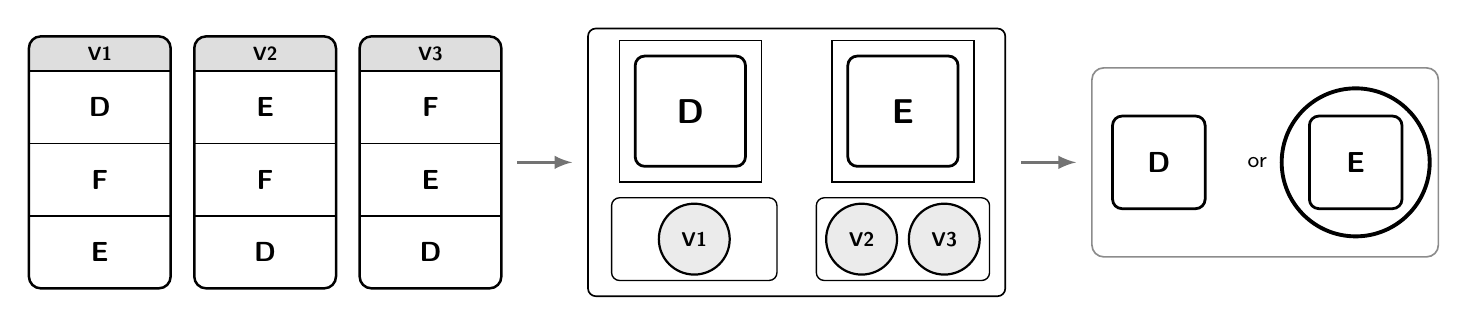
\begin{tikzpicture}[x=1mm,y=1mm]
  % input: the launch cards
  \card{0}{0}{0.4}{V1}{D}{F}{E}
  \card{21}{0}{0.4}{V2}{E}{F}{D}
  \card{42}{0}{0.4}{V3}{F}{E}{D}
  \arr{62}{69}{-16}
  % intermediate: D or E on the tally mat, tokens in the wells
  \draw[line width=0.6pt,rounded corners=1mm] (71,1) rectangle (124,-33);
  \draw[line width=0.5pt] (84-9,-0.5) rectangle (84+9,-18.5);
  \draw[line width=0.5pt] (111-9,-0.5) rectangle (111+9,-18.5);
  \tile{84}{-9.5}{0.5}{D}
  \tile{111}{-9.5}{0.5}{E}
  \draw[line width=0.5pt,rounded corners=1mm] (74,-20.5) rectangle (95,-31);
  \draw[line width=0.5pt,rounded corners=1mm] (100,-20.5) rectangle (122,-31);
  \token{84.5}{-25.75}{0.5}{V1}
  \token{105.75}{-25.75}{0.5}{V2}
  \token{116.25}{-25.75}{0.5}{V3}
  \arr{126}{133}{-16}
  % output: the winner circled, as in Problem 1
  \draw[line width=0.6pt,black!45,rounded corners=1.5mm] (135,-4) rectangle (179,-28);
  \tile{143.5}{-16}{0.42}{D}
  \node at (156,-16) {\footnotesize or};
  \tile{168.5}{-16}{0.42}{E}
  \ring{168.5}{-16}{9.4}
\end{tikzpicture}
\end{center}

\vspace{12mm}
\prob{1}Use cards V1, V2 and V3 for each vote below. Circle the winner.

\vspace{8mm}
\begin{center}
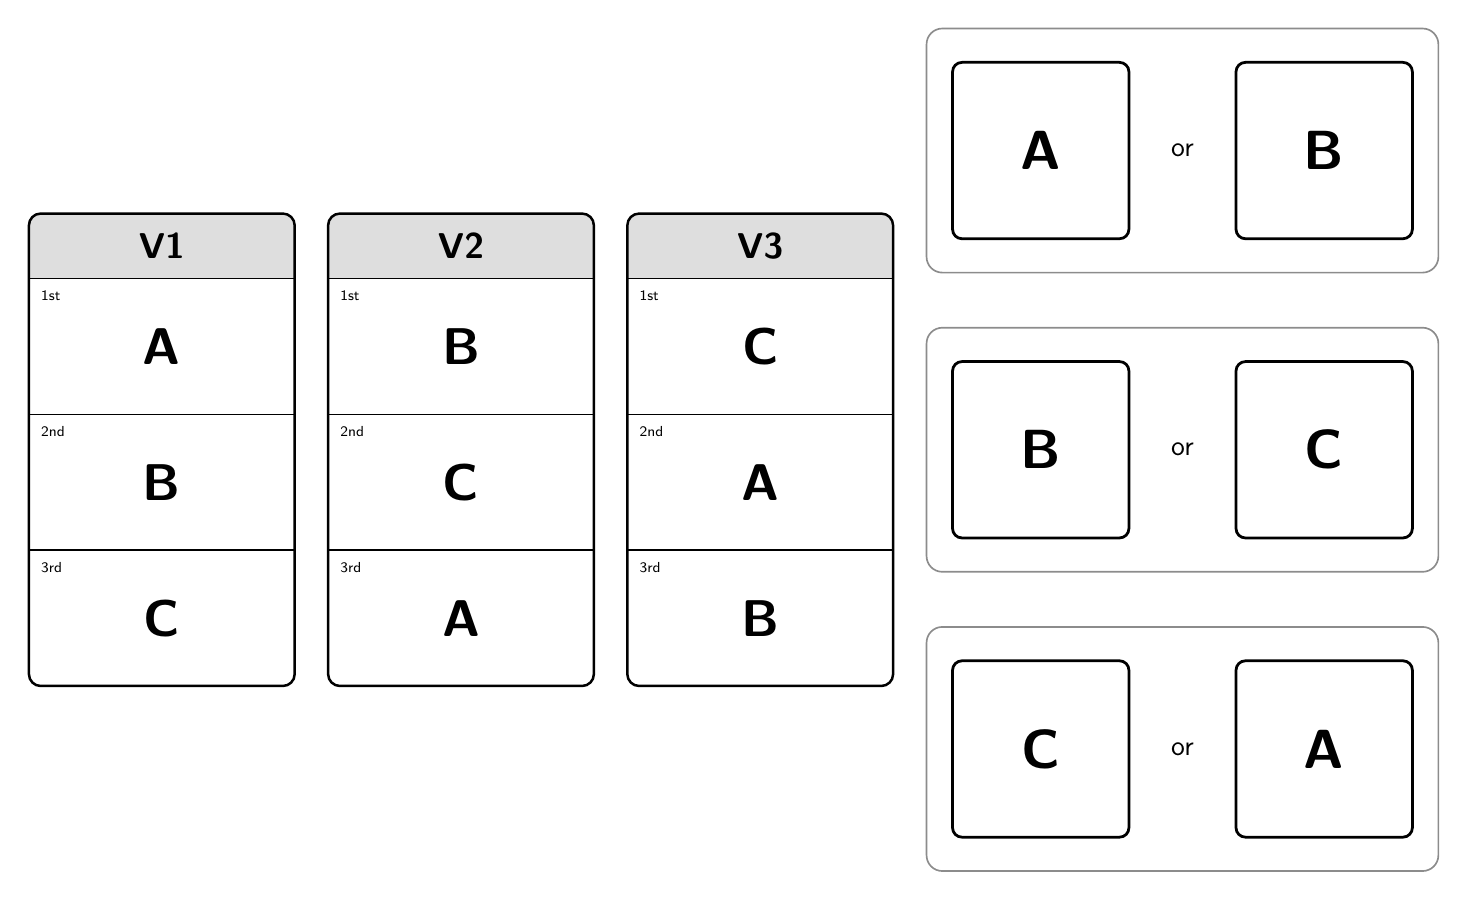
\begin{tikzpicture}[x=1mm,y=1mm]
  \card{0}{-23.5}{0.75}{V1}{A}{B}{C}
  \card{38}{-23.5}{0.75}{V2}{B}{C}{A}
  \card{76}{-23.5}{0.75}{V3}{C}{A}{B}
  \foreach \y/\p/\q in {0/A/B, -38/B/C, -76/C/A} {
    \draw[line width=0.6pt,black!45,rounded corners=2mm] (114,\y) rectangle (179,\y-31);
    \tile{128.5}{\y-15.5}{0.8}{\p}
    \node at (146.5,\y-15.5) {or};
    \tile{164.5}{\y-15.5}{0.8}{\q}
  }
\end{tikzpicture}
\end{center}

\newpage
% ======================= Page 2 =======================
\prob{2}In a knockout, the cards vote on the first pair of letters. Then they
vote between that winner and the letter that waited.

\medskip
\begin{center}
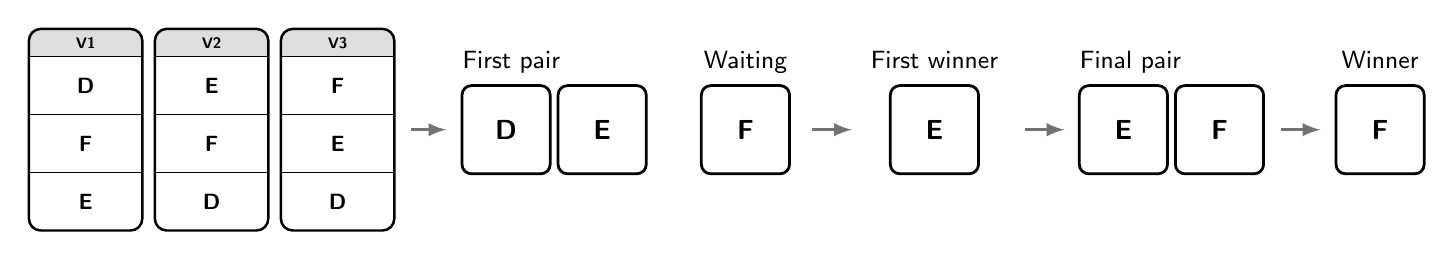
\begin{tikzpicture}[x=1mm,y=1mm]
  % input: the launch cards again
  \card{0}{0}{0.32}{V1}{D}{F}{E}
  \card{16}{0}{0.32}{V2}{E}{F}{D}
  \card{32}{0}{0.32}{V3}{F}{E}{D}
  \arr{48.5}{53}{-12.8}
  % start: first pair D E, F waiting
  \matlabel{55}{-5}{base west}{First pair}
  \tile{60.6}{-12.8}{0.4}{D}
  \tile{72.8}{-12.8}{0.4}{E}
  \matlabel{91}{-5}{base}{Waiting}
  \tile{91}{-12.8}{0.4}{F}
  \arr{99.5}{104.5}{-12.8}
  % intermediate: E wins the first vote
  \matlabel{115}{-5}{base}{First winner}
  \tile{115}{-12.8}{0.4}{E}
  \arr{126.5}{131.5}{-12.8}
  % E against the letter that waited
  \matlabel{133.4}{-5}{base west}{Final pair}
  \tile{139}{-12.8}{0.4}{E}
  \tile{151.2}{-12.8}{0.4}{F}
  \arr{159}{164}{-12.8}
  % output
  \matlabel{171.6}{-5}{base}{Winner}
  \tile{171.6}{-12.8}{0.4}{F}
\end{tikzpicture}
\end{center}

\medskip
Run each knockout below on the knockout mat with cards V1, V2 and V3.
Circle the winner.

\vspace{12mm}
\begin{center}
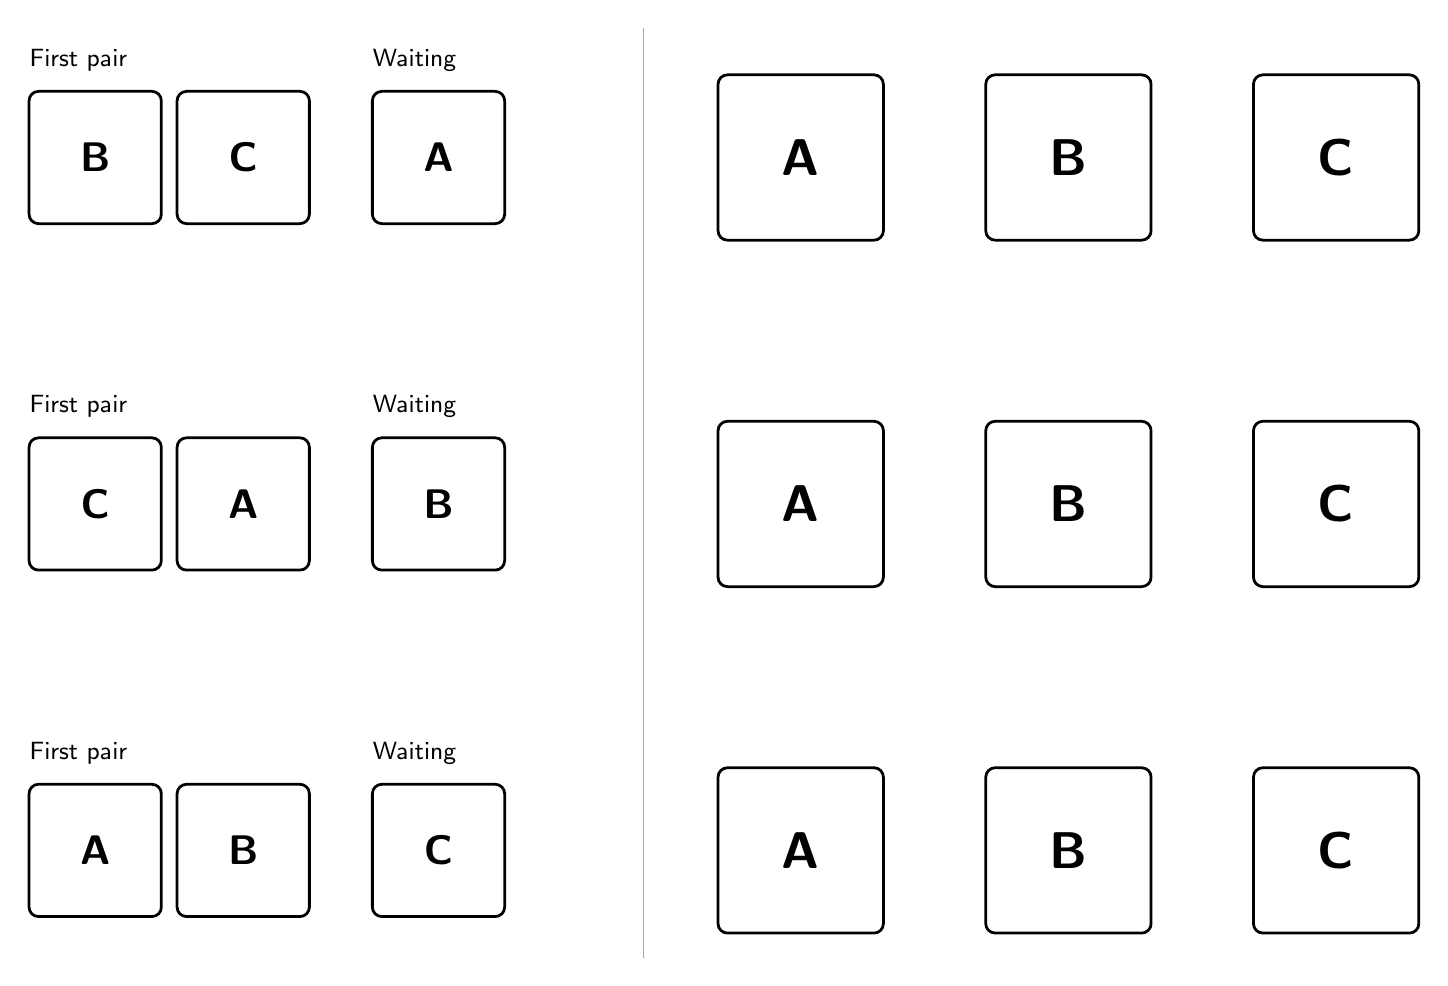
\begin{tikzpicture}[x=1mm,y=1mm]
  \foreach \y/\p/\q/\w in {0/B/C/A, -44/C/A/B, -88/A/B/C} {
    \kostart{0}{\y}{\p}{\q}{\w}
    \abcrow{132}{\y-10.4}
  }
  \draw[line width=0.5pt,black!35] (78,6)--(78,-112);
\end{tikzpicture}
\end{center}

\newpage
% ======================= Page 3 =======================
\prob{3}Use these cards instead of yours. Which letters can win a knockout?
Circle each one.

\vspace{10mm}
\begin{center}
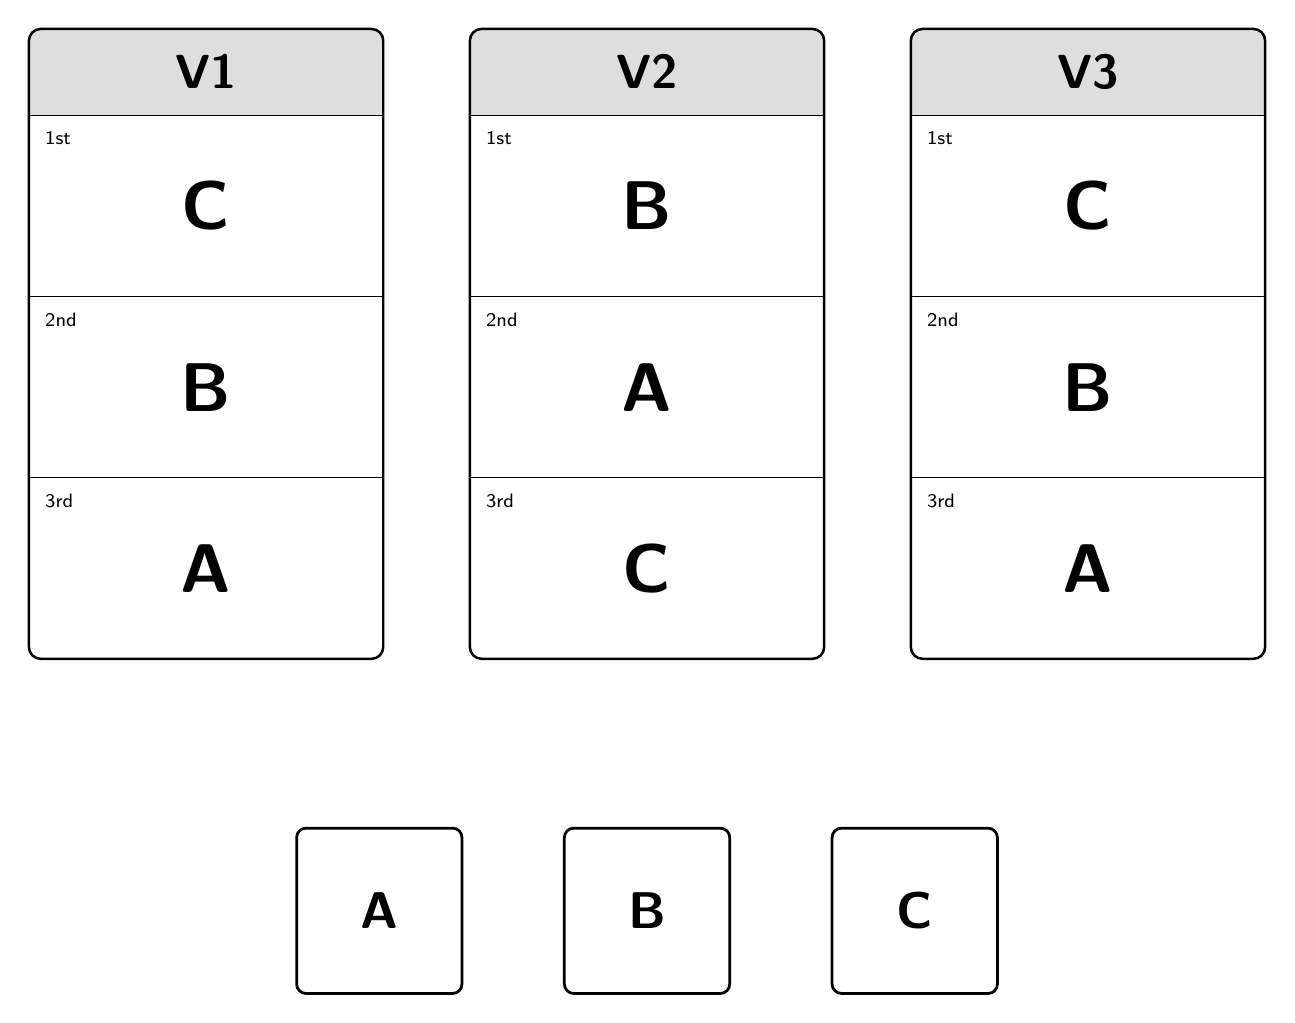
\begin{tikzpicture}[x=1mm,y=1mm]
  \card{0}{0}{1}{V1}{C}{B}{A}
  \card{56}{0}{1}{V2}{B}{A}{C}
  \card{112}{0}{1}{V3}{C}{B}{A}
  \abcrow{78.5}{-112}
\end{tikzpicture}
\end{center}

\newpage
% ======================= Page 4 =======================
\prob{4}Use these cards instead of yours. Which letters can win a knockout?
Circle each one.

\vspace{10mm}
\begin{center}
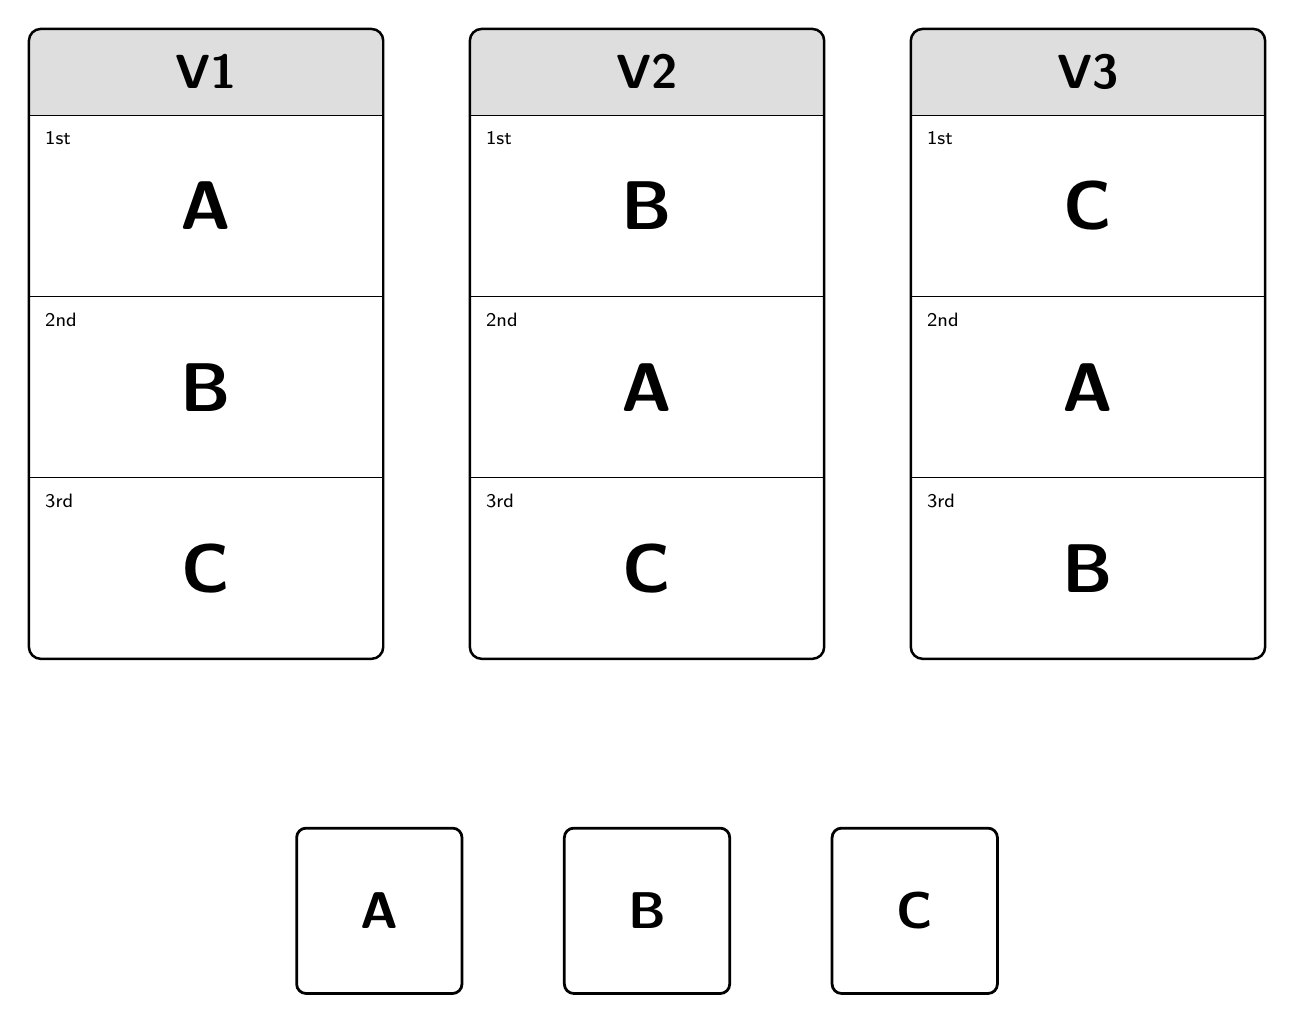
\begin{tikzpicture}[x=1mm,y=1mm]
  \card{0}{0}{1}{V1}{A}{B}{C}
  \card{56}{0}{1}{V2}{B}{A}{C}
  \card{112}{0}{1}{V3}{C}{A}{B}
  \abcrow{78.5}{-112}
\end{tikzpicture}
\end{center}

\newpage
% ======================= Page 5 =======================
\prob{5}Swap two letters on one of these cards so that C wins, no matter which
letter waits. Make the new card from a blank card and letter slips.

\vspace{6mm}
\begin{center}
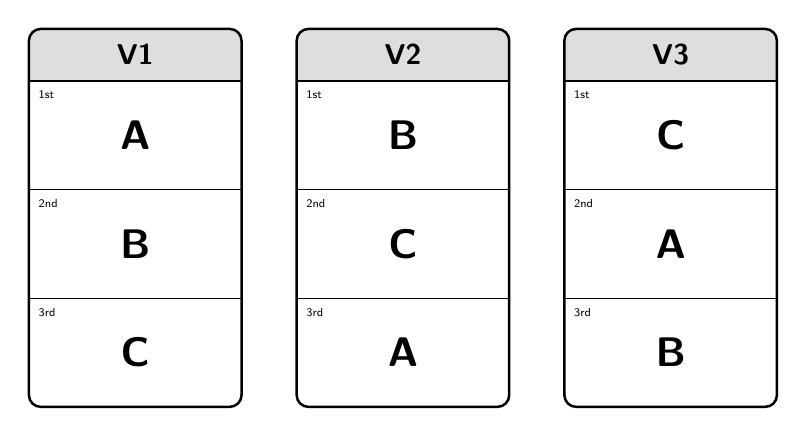
\begin{tikzpicture}[x=1mm,y=1mm]
  \card{0}{0}{0.6}{V1}{A}{B}{C}
  \card{34}{0}{0.6}{V2}{B}{C}{A}
  \card{68}{0}{0.6}{V3}{C}{A}{B}
\end{tikzpicture}
\end{center}

\vspace{22mm}
\prob{6}Build three new cards V1, V2 and V3 from blank cards and letter slips,
with one A, one B and one C on each card. Make B win, no matter which letter waits.

\vspace{8mm}
\begin{center}
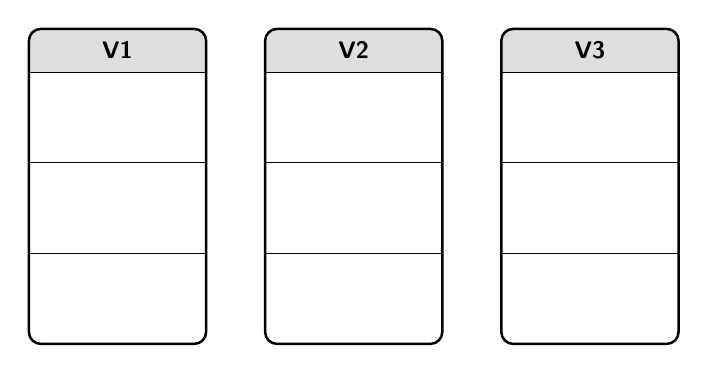
\begin{tikzpicture}[x=1mm,y=1mm]
  \frames{0}{0}
\end{tikzpicture}
\end{center}

\newpage
% ======================= Page 6 =======================
\prob{7}Build three cards the same way, with B 1st on just one card. Make B win,
no matter which letter waits, or use the cards to show why you can't.

\vspace{8mm}
\begin{center}
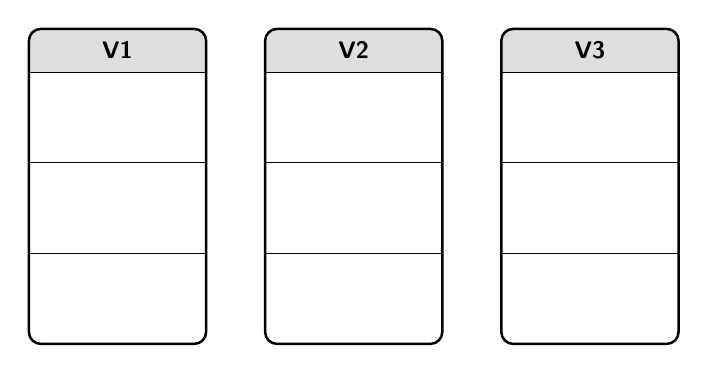
\begin{tikzpicture}[x=1mm,y=1mm]
  \frames{0}{0}
\end{tikzpicture}
\end{center}

\vspace{22mm}
\prob{8}Build three cards the same way, with B never 1st. Make B win, no matter
which letter waits, or use the cards to show why you can't.

\vspace{8mm}
\begin{center}
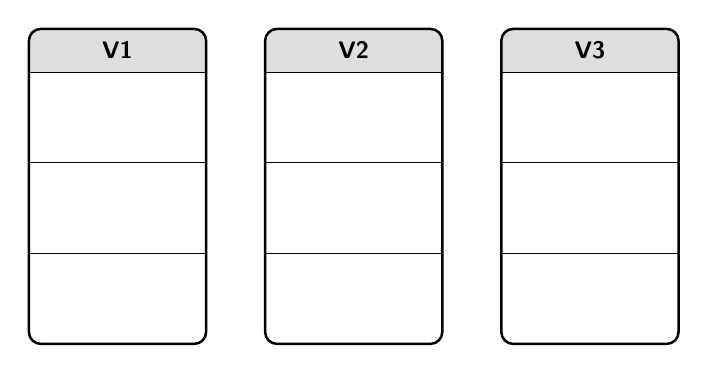
\begin{tikzpicture}[x=1mm,y=1mm]
  \frames{0}{0}
\end{tikzpicture}
\end{center}

\end{document}
